
\documentclass[11pt]{article}
\usepackage{graphicx}
\begin{document}

\section{
Geometron Presents Geometron}

\begin{figure}

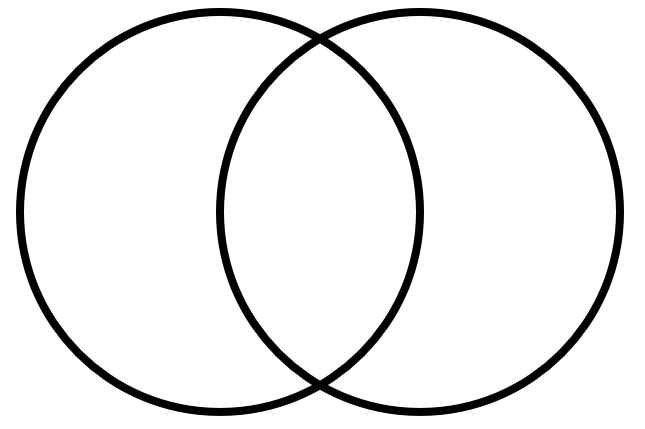
\includegraphics[width=\linewidth]{../figures/vesica.png}

\caption{Vesica Pisces.  The "hello, world" of geometric languages}
\end{figure}


\begin{figure}

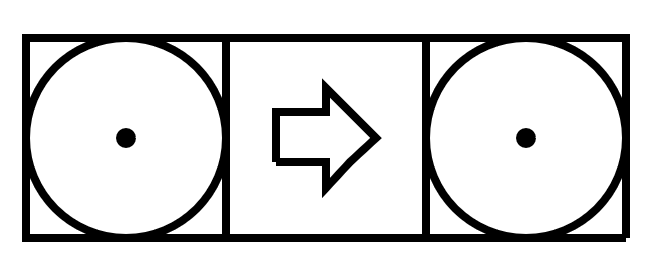
\includegraphics[width=\linewidth]{../figures/vesicacode.png}

\caption{Symbols which spell out the vesica pisces. Each symbol represents a geometric action, and they are: draw circle of radius "side", move right by "side", draw circle of radius "side".}
\end{figure}


\end{document}
